%% Special GenAICHI Settings and Setup
% \documentclass[manuscript,screen,nonacm]{acmart}
\documentclass[manuscript,review,anonymous]{acmart}
% \acmConference[]{} % need to include this to suppress addresses footer

\begin{document}

\title{Design Patterns for Intelligent Musical Instruments: Case Studies in Performance with IMPSYpi}

\author{Charles Patrick Martin}
\email{charles.martin@anu.edu.au}
\orcid{0000-0001-5683-7529}
\affiliation{%
  \institution{The Australian National University}
  \city{Canberra}
  \state{ACT}
  \country{Australia}
}


\begin{abstract}
This paper is about making a cheap minimal battery-powered AI music controller, the GenAI MIDI Plug, that can be integrated into regular electronic music setups for exploring human-AI collaboration.
While machine generation of symbolic music and digital audio are hot topics there have been relatively few digital musical instruments that integrate generative AI, partly due to the complexity of training and deploying artist-centered generative AI systems.
This research introduces a minimal design for a generative AI controller based on an inexpensive single board computer that connects via MIDI to other musical devices.
Our approach uses a small artist-collected dataset that can be trained on a regular computer and very few hardware components.
This work demonstrates that real generative AI can occur on low-end hardware in an interactive music performance context. 
This system could be applied by a wide community of musicians and instrument designers to experiment with new intelligent musical instrument prototypes.
\end{abstract}

\keywords{generative AI, small data, human-AI interaction, intelligent musical instruments}

% \ccsdesc[500]{Applied computing~Sound and music computing}
% \ccsdesc[300]{Human-centered computing~Ubiquitous and mobile computing systems and tools}
% \ccsdesc[300]{Computing methodologies~Neural networks}
% \printccsdesc

\maketitle

\section{Introduction}\label{intro}

This paper explores how generative AI may be embedded within interactive musical systems for live performance through a series of case study instruments and performances where hardware and software synthesisers and instruments have been coupled with a Linux-based single board computer pre-loaded with generative AI software.
A broad range of NIME research has applied AI techniques, and in particular deep learning, for tasks such as mapping, audio or sensor analysis and musical data generation~\cite{jourdan_nime_ml_review}. While the analysis of gestures~\cite{visi_iml_gesture} remains a popular application, deep learning models now enable generation of audio~\cite{caillon_rave}, symbolic music~\cite{symbolicmusic2023}, and interaction~\cite{Martin2019} data.
Despite this wide range of research, relatively few intelligent musical instruments, that is, digital musical instruments (DMIs) integrating generative AI, are available to be used in ordinary musical practice.
The goal of this research is to open the design space of intelligent musical instruments by proposing an approach to creating such systems that is cheap, minimal, and battery-powered, thus enabling integration into a wider variety of musical systems by a diverse population of artists and experimenters. 
Our IMPSYpi system includes an implementation of a mixture density recurrent neural network (MDRNN), appropriate for generating expressive musical signals from small artist-centered datasets. 
This system can communicate to existing software and hardware musical systems using MIDI over USB, standard MIDI hardware connections, as well as OSC or WebSockets over a network.
In this way, existing musical systems can be integrated with a generative AI system to create an intelligent musical instrument that can play by itself or take turns with and adapt to a human performer's input.
In this research we introduce IMPSYpi and explore it's potential through a number of case studies of intelligent musical instruments used in our artistic research.
Our experiments show that this idea is feasible and useful for experimenting with human-AI musical interaction.
We distill lessons learned through ideation, development and performance with these systems to propose design recommendations for future intelligent musical instruments.
This work could serve as a basis for prototyping further intelligent musical instruments and exploring their application in different creative practices.

Research applying generative AI on single board computers promises to allow these technologies to be embedded within self-contained musical instruments. 
This has been demonstrated for Raspberry Pi~\cite{Naess:2019aa, martin_empi} and Bela~\cite{pelinski_pipeline_bela} platforms. 
Previous work has acknowledged the difficulties faced by instruments builders wishing to embed AI within new instruments in terms of data collection and training~\cite{Martin2019} and cross-compiling code~\cite{pelinski_pipeline_bela}. These efforts are  mirrored in other creative design fields~\cite{teachablemachine}.
In contrast with very large and costly industrial-scale AI, these projects have emphasised a small data~\cite{Vigliensoni:2022} mindset where artists should collect, curate, train, and deploy their own AI systems. 

Jourdan and Caramiaux have identified gaps in interactivity and practice~\cite{jourdan_nime_ml_review} in AI-supported musical expression, particularly where deep learning is applied. 
They argued that as deep learning systems have become more complex there have been fewer examples of application in long-term musical practice and artists have less interaction with data collection and training phases. 
This contrasts with earlier parameter-mapping approaches where long term practice has been studied~\cite{fiebrink_years_ml}.
A small data approach to deep learning may only be part of the solution. 
It could be that engaging artists with simpler prototype systems that can be easily integrated into their existing practice could lead to more opportunities for data collection, training, and long-term practice.

Framing a generative AI instrument as a MIDI plug leverages musicians' existing significant skills and understanding of their instruments which could allow a deeper co-creative practice with an AI system.
The present paper documents the process of creating our GenAI MIDI Plug showing that it is feasible, affordable and achievable for non-experts in AI. 
This process has also revealed pain points in setting up a generative AI instrument and new possibilities for co-creation that might encourage more widespread prototyping, hacking, and musicking with AI in NIMEs.

\section{Background}\label{background}

\subsection{Generative AI in Performance}

\subsection{Embedded Musical Instruments}

\subsection{Research Methods}



\section{System Design}\label{sys-design}

% Update this to relate specifically to IMPSYpi and the different connectivity methods.
% This shouldn't go too much into specific examples, just explain how the system works.


The GenAI MIDI Plug system consists of Python software and a minimal hardware setup that able to run the generative AI software and communicate MIDI messages to an external electronic music device. Unlike other embedded music systems, this setup is not intended to produce sound but simply control other electronic music devices so the single board computer does not need to have an audio output. To support our design goals of minimal size and price but with good support for other instrument designers a Raspberry Pi Zero 2 W was used in our project. This single board computer includes a quad-core 64-bit ARM Cortex-A53 at 1GHz with 512MB of RAM. This board meets the cost (15USD as of 2024) and size (65mm x 30mm) requirements. Crucially, it is able to run the 64-bit Raspberry Pi OS ensuring good compatibility with machine learning libraries for Python. The Pi is configured to run our software on boot.

The hardware setup is shown in Figure \ref{fig:system-photo} and consists of a Raspberry Pi Zero 2 W and standard enclosure, a 16GB microSD card and MIDI (5-pin DIN) connector. The MIDI connector is linked via a short cable to the Raspberry Pi and soldered directly to GPIO pads corresponding to the Pi's serial (UART) output. Providing a MIDI output from the Pi's 3.3V signals is straightforward requiring only two resistors~\cite{MIDI-Manufacturers-Association:2014aa}: 10$\Omega$ between the UART TX pin and pin 5 on the MIDI connector and 33$\Omega$ between the 3.3V output and MIDI pin 4. MIDI pin 2 is connected to ground. In our setup, the resistors are concealed within the MIDI connector.

\begin{figure}
    \centering
    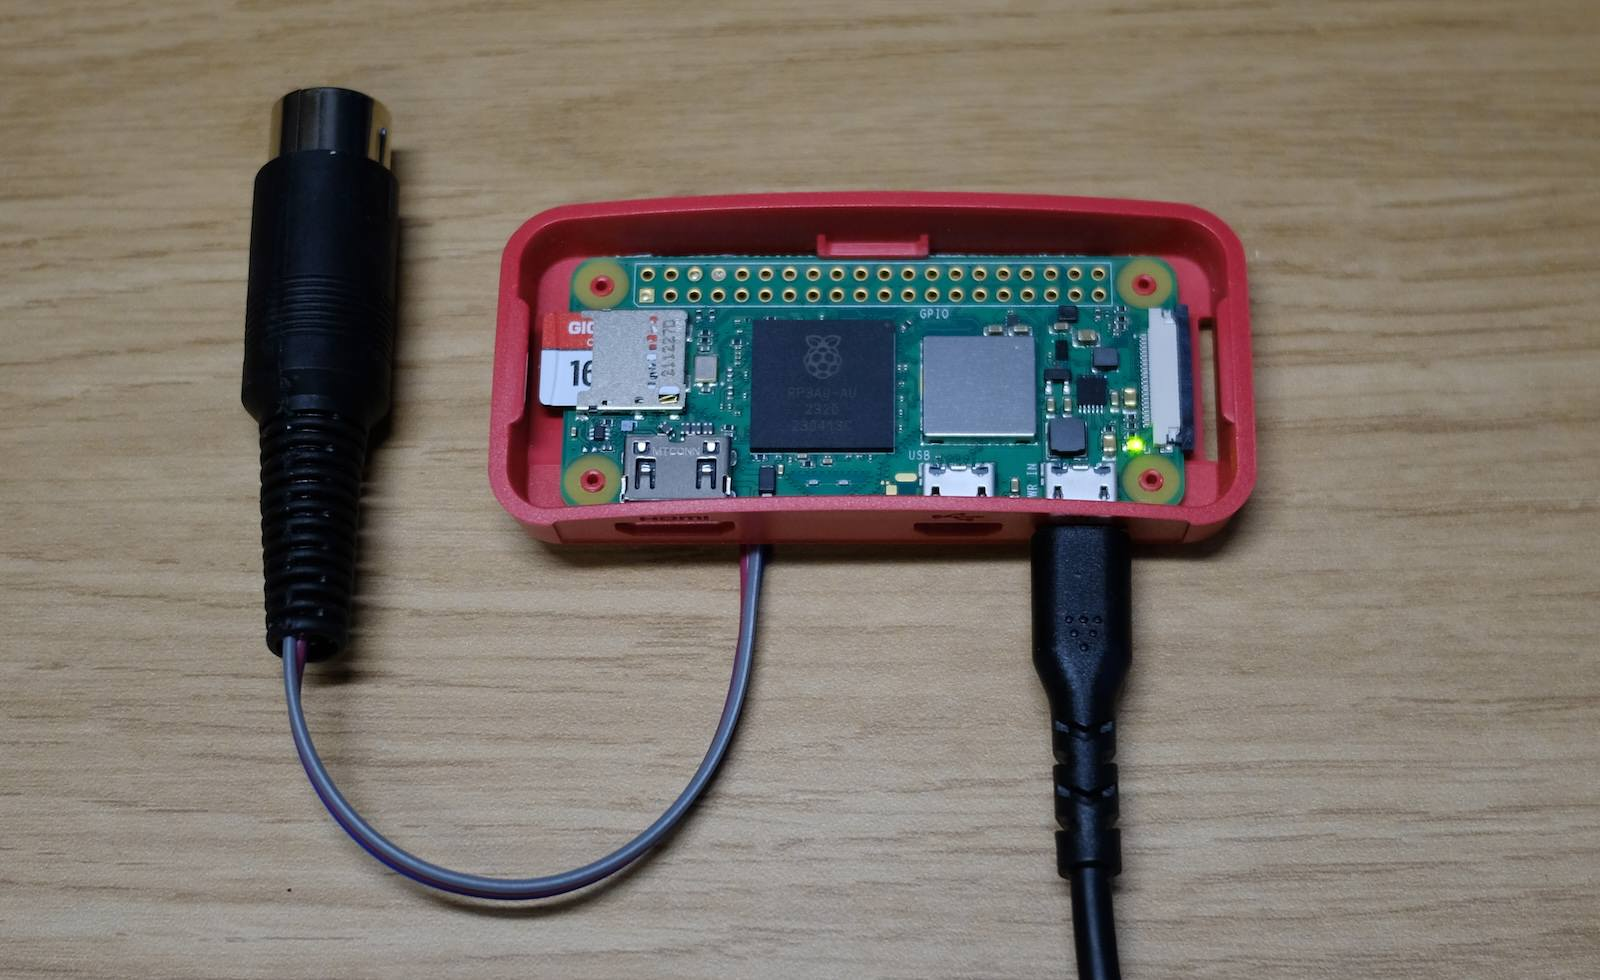
\includegraphics[width=\columnwidth]{figures/desk-shot.jpg}
    \caption{The GenAI MIDI Plug with cover removed. The hardware consists of a Raspberry Pi Zero 2 W with case, 16GB microSD card, and a MIDI connector soldered directly to the Raspberry Pi.}
    \label{fig:system-photo}
\end{figure}

The software part of our system is a Python program running on the Raspberry Pi that generates musical data and sends it via a serial connection to an external MIDI-enabled electronic musical instrument.
Following Martin and Torresen~\cite{Martin2019}, we use a mixture density recurrent neural network (MDRNN) as the machine learning paradigm for generating a stream of musical data and we apply the Keras-MDN-Layer library~\cite{keras-mdn-layer} to construct this neural network.

Our system uses a two dimensional MDRNN that generates pairs of data that we interpret as a musical value and time delta for when that value should occur in the future. 
The network is autoregressive, so takes the preceding value as input to the generate next, but it is also recurrent, so it stores a lossy history of generated values using LSTM units. 
Our MDRNN model is configured to use 2 layers of 32 LSTM units. Although this is a very small number of parameters compared to industrial generative AI and large language models, it is sufficient for generating musically useful data in real-time on small hardware.

\begin{figure}
    \centering
    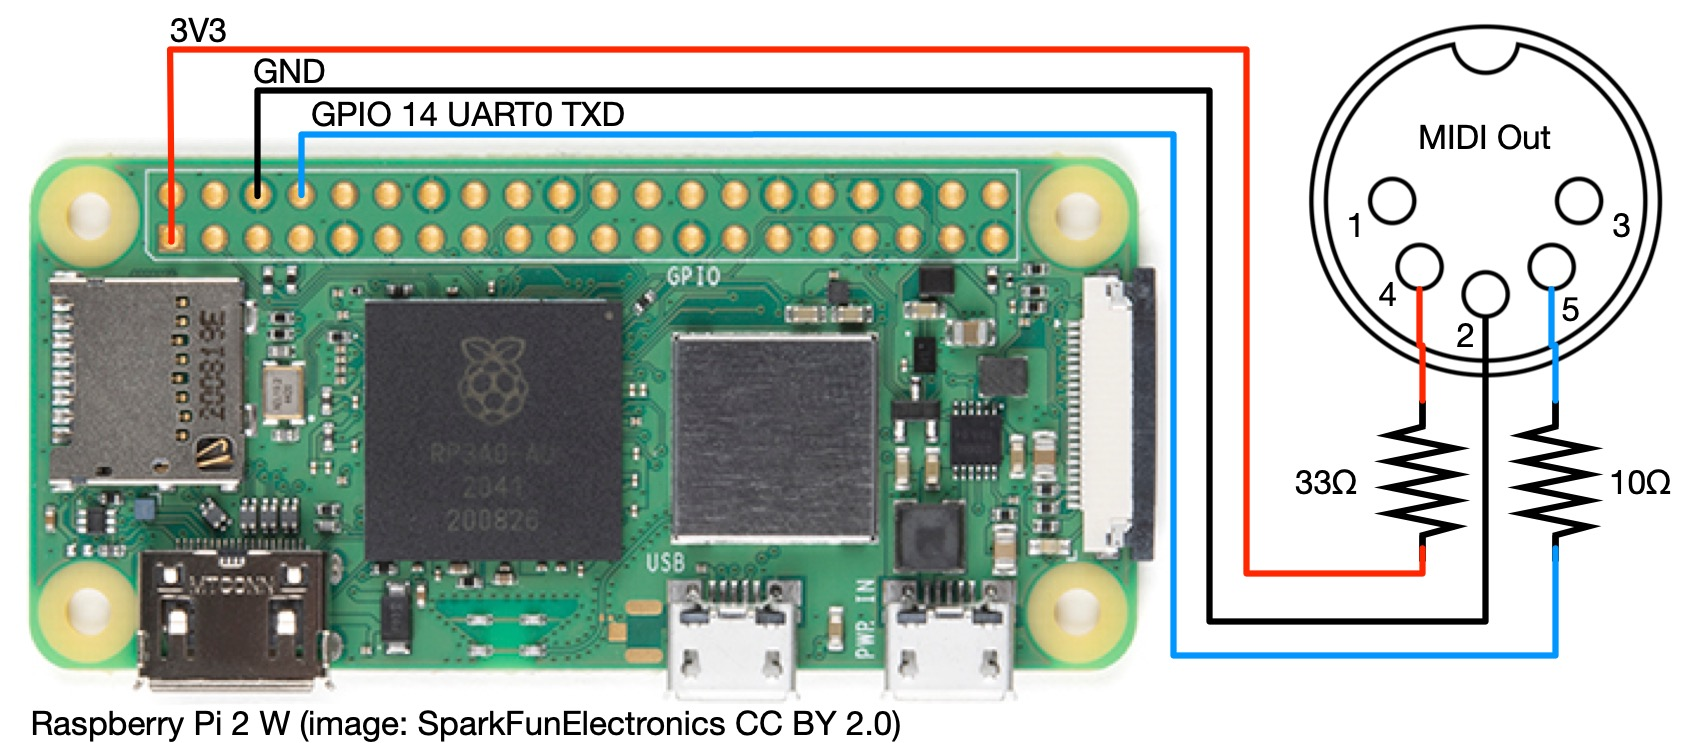
\includegraphics[width=\columnwidth]{figures/sf-image.jpg}
    \caption{Circuit diagram for the GenAI MIDI Plug. A MIDI output can be obtained from a Raspberry Pi with the addition of only two resistors that can be concealed inside the MIDI connector.}
    \label{fig:enter-label}
\end{figure}

\section{Case Studies}\label{case-studies}

In this section we describe case studies where we have used IMPSYpi to create intelligent musical instruments and performed with them in live concerts. We have applied an exploratory and autobiographical artistic research approach where these instruments have been developed for our own use and tested in authentic live performance situations.

\subsection{The Self-Playing Volca}

\begin{figure}
    \centering
    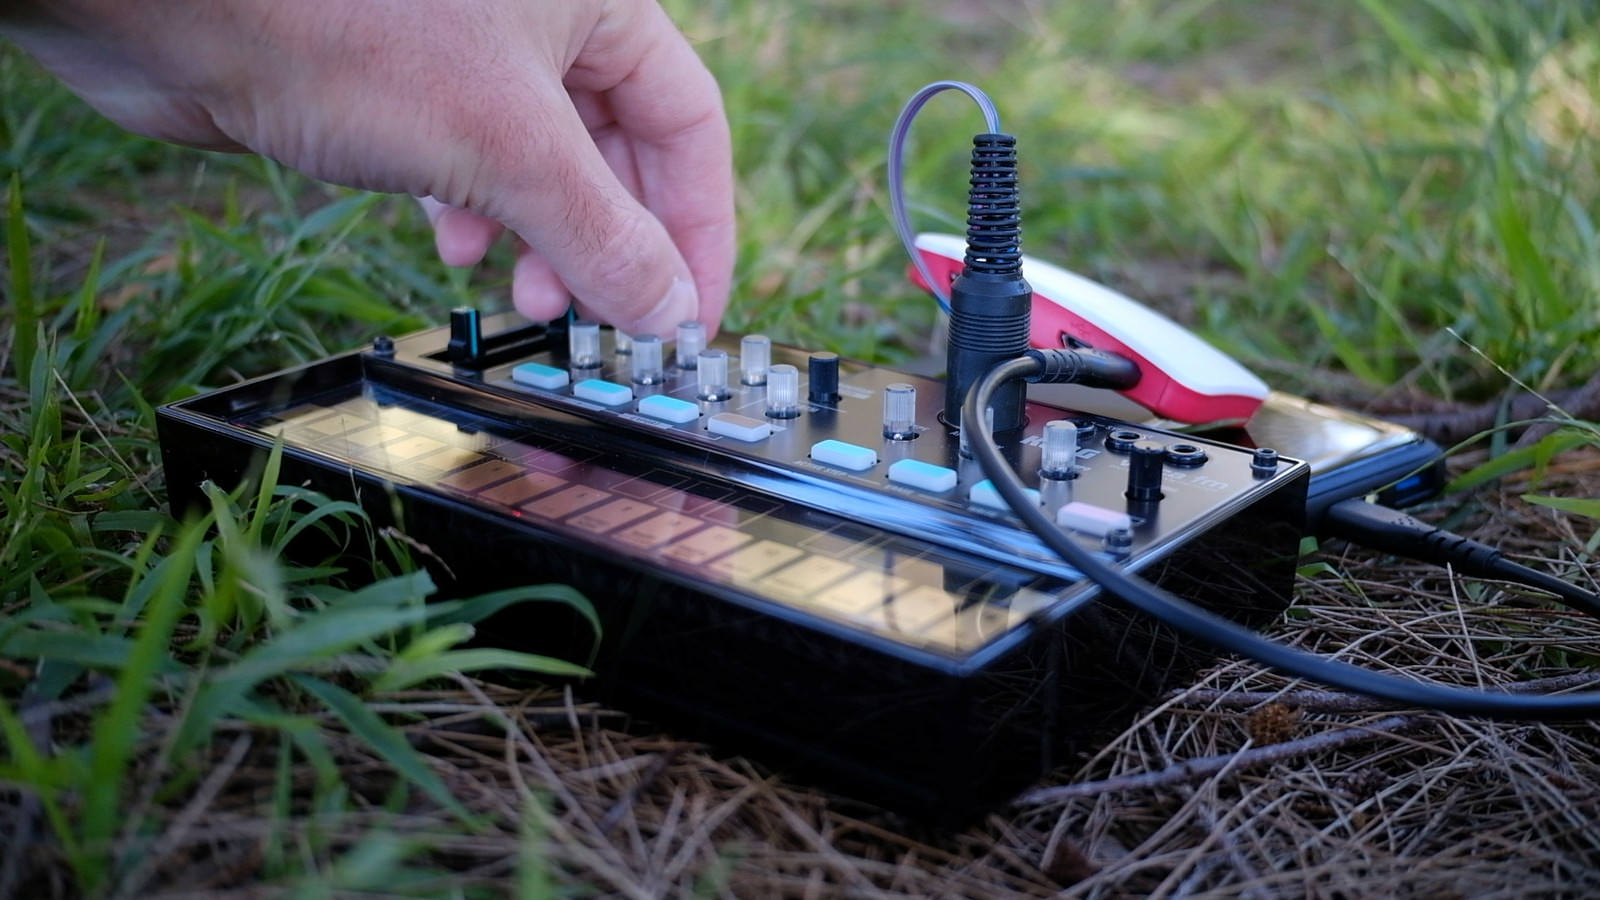
\includegraphics[width=\columnwidth]{figures/outside-1.jpg}
    \caption{Battery-powered human-AI interaction on a Korg Volca FM. The generative AI system running on the Raspberry Pi Zero controls pitch and rhythm via the MIDI connector while the musician edits the synth patch. Video: \url{https://vimeo.com/911078203}}
    \label{fig:self-playing-volca}
\end{figure}

The self-playing Volca was a proof-of-concept design to establish whether real-time generative-AI MIDI signals from the Raspberry Pi Zero was feasible and musically interesting.
For this design, a simple MIDI output was obtained from the Raspberry Pi's GPIO header UART pins.
The output was connected to the battery-powered Volca FM and the Raspberry Pi itself was powered by a USB power bank.
Initially, only pitch and rhythm was controlled by the IMPSYpi.
The MDRNN was trained on a corpus of 65 minutes of musical human interaction with a single continuous controller. This corresponded to around 75000 interaction events (value and time delta).
The corpus consisted of data with continuously changing values between 0 and 1 and time deltas recorded in seconds. This is somewhat different to melodic MIDI note data that is often used in musical AI. 
The MDRNN output (0.0--1.0) was converted to a MIDI pitch value from 0--127 and a corresponding MIDI note-on message scheduled to be sent at the time-delta generated by the MDRNN.

This initial experiment emphasised portability with a completely self-contained and battery-powered system: the Volca FM even has an internal speaker.
While the MDRNN could play notes, and a human performer could adjust the synthesiser's timbre or settings as well as play overlapping notes on the keyboard, the MDRNN couldn't respond to the performer as the Volca FM does not have a MIDI output.
This meant that although this experiment started to explore different roles for the human and MDRNN in controlling the synth, the interaction was necessarily one way.

This experiment also showed that musical performance of the MDRNN when transformed to MIDI note-on commands is quite different from other generative AI MIDI performance systems. Traditionally , AI MIDI systems are trained on compositions or melodies, while this system was trained on expressive interaction with a continuous controlled. 
The resulting performances are include glissandi of various speeds, starting points, and lengths.
Sent through the Volca FM, these can sound unusual as the synthesiser retriggers it's envelope for each note.
This dataset may be more applicable to synthesis parameter control tasks where a musician would like a particular value to change smoothly in an expressive way including varying speed and pauses.


\subsection{The Intelligent MicroFreak and S-1}

\begin{figure}
	\centering
	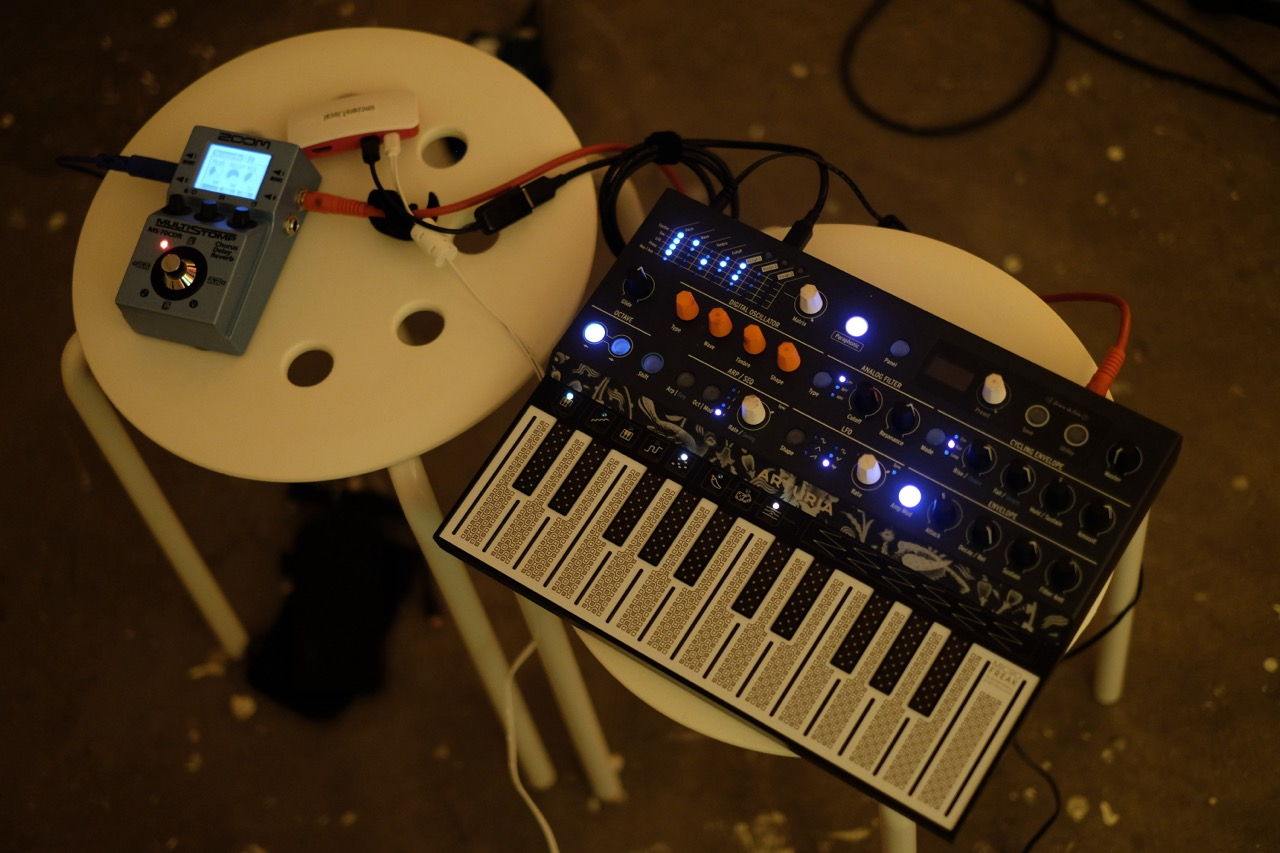
\includegraphics[width=\columnwidth]{figures/intelligent-microfreak.jpg}
	\caption{}
	\label{fig:microfreak}
\end{figure}

\begin{figure}
	\centering
	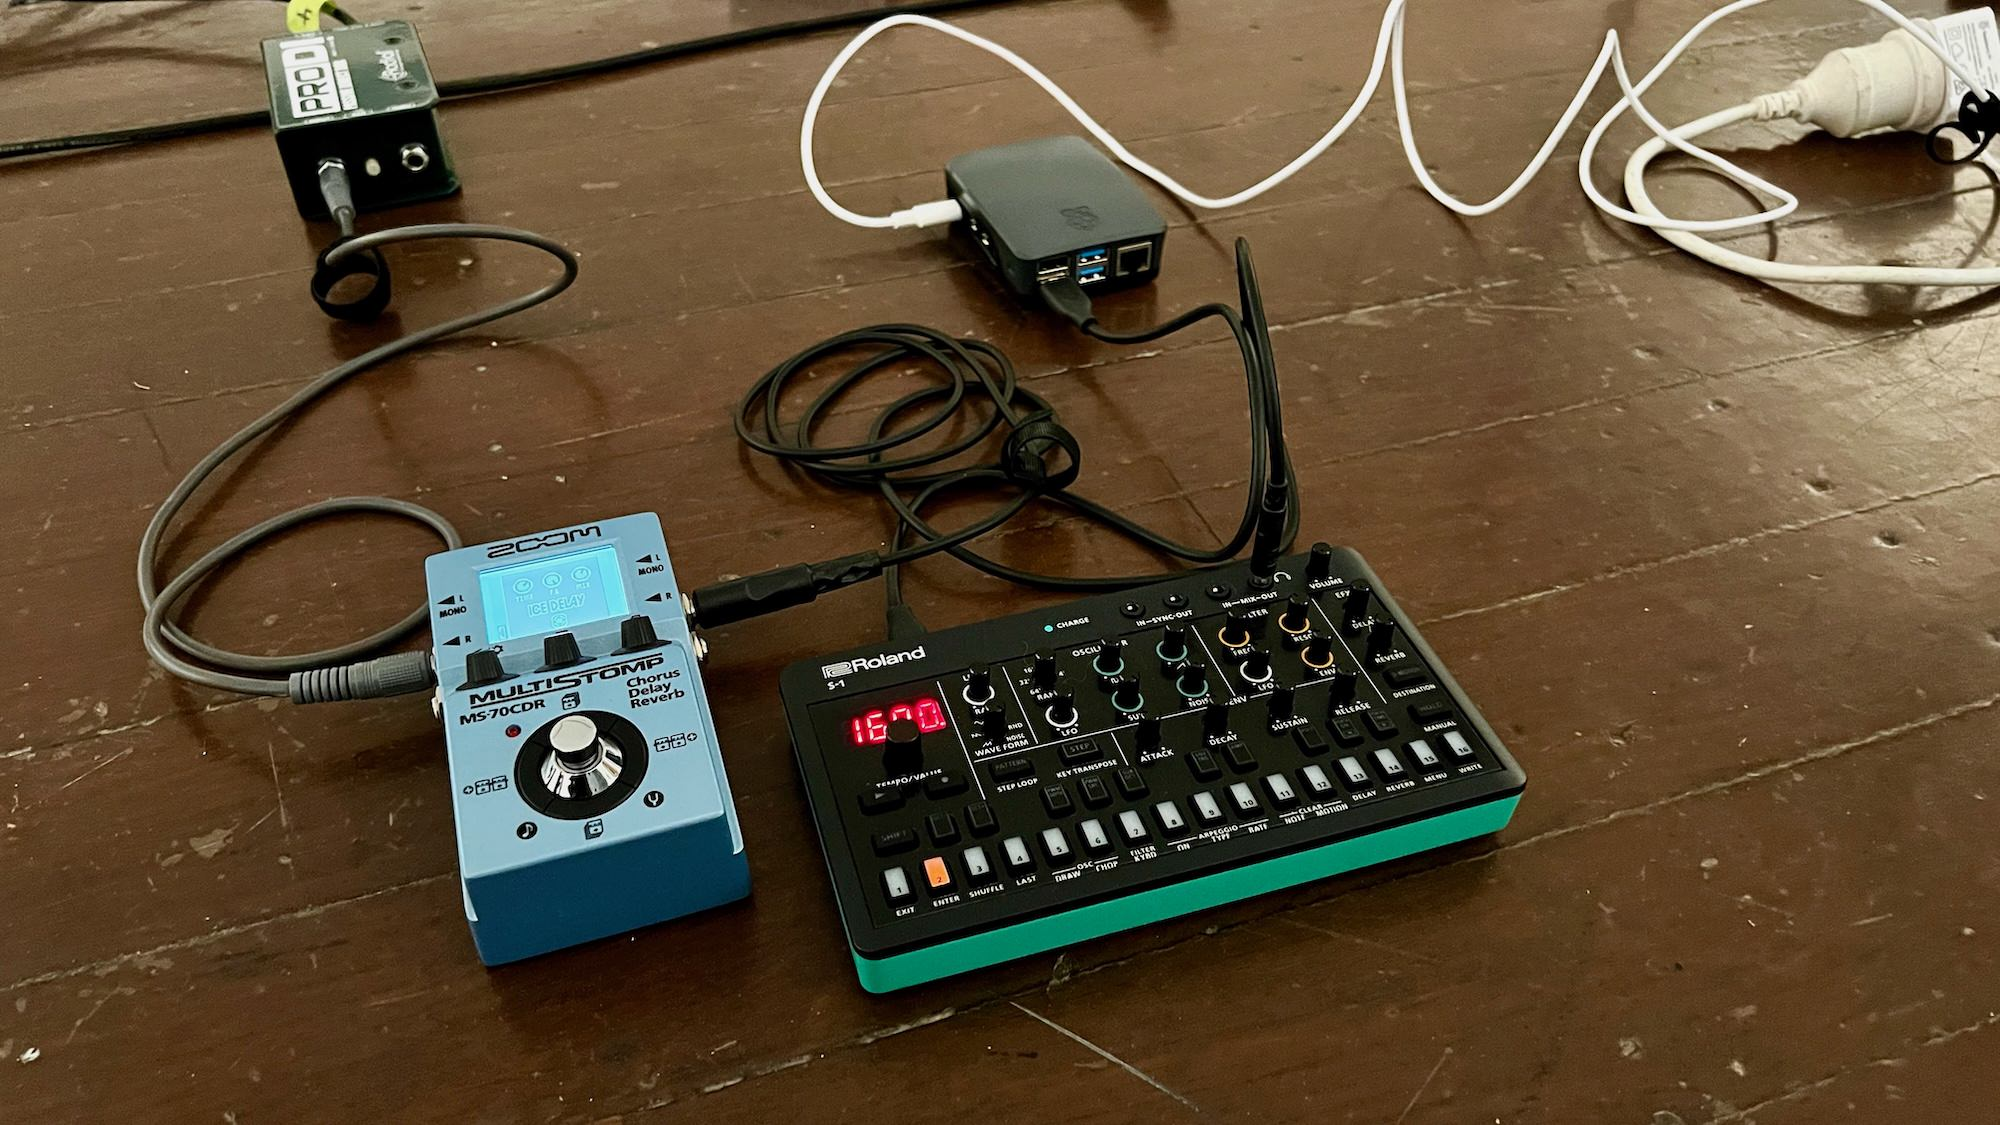
\includegraphics[width=\columnwidth]{figures/intelligent-s-1.jpg}
	\caption{}
	\label{fig:s-1}
\end{figure}

While the above example demonstrated one-way input from IMPSYpi into a hardware synthesiser, other systems promised to support two-way interaction. 
Establishing a MIDI-over-USB connection between IMPSYpi and a hardware synth often allows physical controls on the synthesiser to send signals to the IMPSYpi while simultaneously controlling the synthesiser.
The IMPSYpi is then configured to behave in a call-and-response manner so that when the human is adjusting the synth controls and playing notes, these IMPSYpi tracks these signals and only when the human stops for a certain amount of time does the IMPSYpi take over the controls. 
This arrangement was first trialled with an Arturia MicroFreak synthesiser with IMPSYpi controlling 8 parameters: note-on messages


\subsection{Off-the-shelf}


\begin{figure}
	\centering
	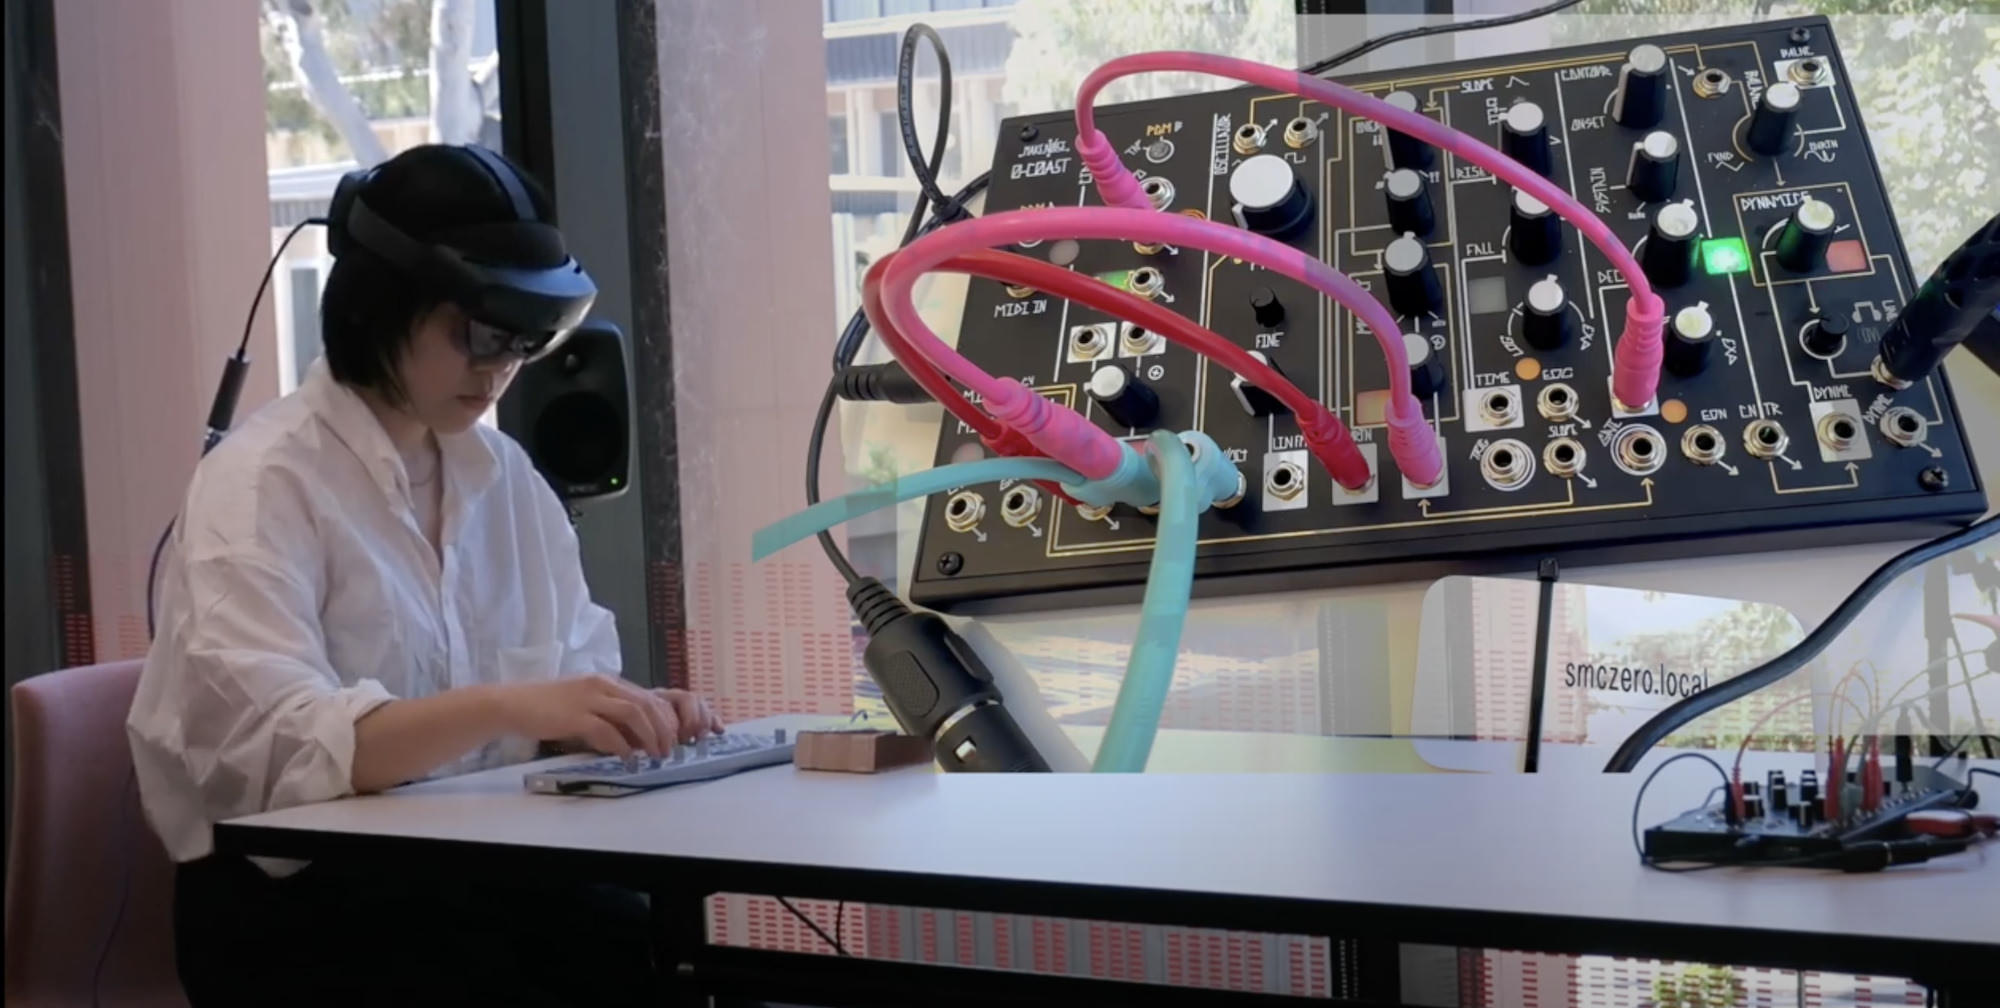
\includegraphics[width=\columnwidth]{figures/off-the-shelf-0coast.jpg}
	\caption{}
	\label{fig:off-the-shelf}
\end{figure}



\subsection{Touching Wires}

\subsection{Intelligent DAWs: Ableton Live and Kymatica AUM}


\section{Discussion}\label{disc}

Our system has been tested in the context of electronic music improvisation where control over a synthesiser is shared between a human and the GenAI MIDI Plug. Figure \ref{fig:human-ai} and our accompanying video\footnote{\url{https://vimeo.com/911078203}} shows excerpts from an outdoor battery-powered improvisation. In this example, the synthesiser is a Korg Volca FM with note values (pitch and rhythm) controlled by the GenAI MIDI Plug. The musician adjusts parameters on the synthesiser patch including pitch shifting the GenAI MIDI signals by octaves.

The experience so far with this system is positive. The signal from the GenAI MIDI Plug can be contextualised as a more expressive and unpredictable kind of LFO (low frequency oscillator) within a synth setup. As it's modelled on human-sourced data, it noodles, pauses, explores different parts of the output range, stops completely sometimes and starts up again at (perhaps) annoying moments. Although it exhibits some behaviours that could be programmed into a hard-coded signal generator it also has a level of stochasticity and variation that that would be more complicated to construct heuristically. Importantly, the very small size of the system means that it can fit into battery-powered electronic music setups. The price of the system means that potentially more than one could be affordably applied in any one performance.

The intention of this research has been not just to create one GenAI MIDI Plug but to demonstrate the feasibility of this approach to instrument designers who may wish to adapt this idea.
The hardware aspects of our system demonstrate a really simple way of connecting a Raspberry Pi Zero to existing electronic music systems. 
Although the software is effective, the Keras MDN Layer~\cite{keras-mdn-layer} library presently requires the full Tensorflow and TensorFlow-Probability libraries. 
The newer 64-bit Raspberry Pi OS should make it easier to install these, but in our experience we were still using a custom build of Tensorflow\footnote{\url{https://github.com/PINTO0309/Tensorflow-bin}} for the Raspberry Pi which may be intimidating for beginners to install. 
Once the system is running, data generation with the MDRNN is quick; however, the process of booting, loading Tensorflow, and starting generation takes around 90 seconds. 
There may be potential to port this system to use lighter libraries (e.g., Tensorflow-Lite) that may load more quickly from boot and could also improve the installation experience for instrument designers.

This work has introduced a minimal approach to creating an intelligent musical instrument, the GenAI MIDI Plug. This research aims to address gaps in creative practice and interaction that have been identified in NIME applications of generative AI. While enabling artist-led data collection and training may support a small-data approach, cheap minimal battery-powered AI music controllers could encourage a greater range of experimentation and prototyping among the wider music community.

\section{Conclusions}\label{concl}


\bibliographystyle{ACM-Reference-Format}
\bibliography{references} 

\end{document}
